% Another chapter whose name you shouldn't ideally change.
\chapter{Results and Discussion}
\section{Results I}
This is how you add a table, just un-comment things and see them work. You can modify the columns and rows and use multi-columns or multi-rows as per your convenience. If you have extremely long tables, I'll suggest to use \textit{longtable} format, just google it.
\begin{table}[ht!]
    \centering
    \begin{tabular}{|c|c|c|c|c|c|c|c|}
        \hline
        N & $f_0$ & $\nu$ & $\epsilon$ & U & L & R & $k_d$ \\
        \hline
        \hline
        64 & 0.35 & $5 \times 10^{-3}$ & 0.166 & 1.0 & 3.86 & 772 & 33.95 \\
        128 & 0.5 & $5 \times 10^{-4}$ & 0.299 & 1.0 & 5.24 & 10470 & 39.32 \\
        \hline
    \end{tabular}
    \caption{Parameters and outputs for the two different runs of forced turbulence}
    \label{param-forced}
\end{table}

\newpage % This is how you force a new page.

\section{Results II}
This is how you combine multiple pics in a grid. You can use \textit{minipage} if there are only a few pictures, but this is to show long array of pictures. \footnote{More about this in \autoref{app-a}.} % This is how you add footnotes.
\subsection{Velocity Field evolution in ABC Forcing}
\begin{figure}[ht!]
\centering
\advance\leftskip-3cm
\advance\rightskip-3cm

\begin{tabular}{llll}

\subfloat[z = 1]{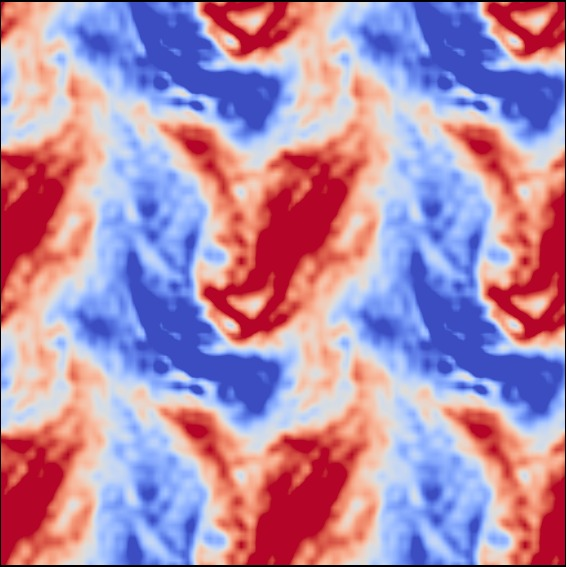
\includegraphics[width=0.2\textwidth]{Figures/ABC/t1z0.jpeg}} & \subfloat[z = 33]{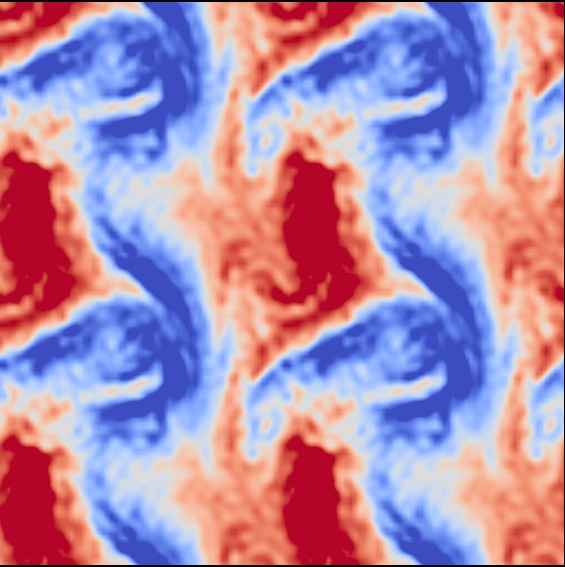
\includegraphics[width=0.2\textwidth]{Figures/ABC/t1z32.jpeg}} & \subfloat[z = 65]{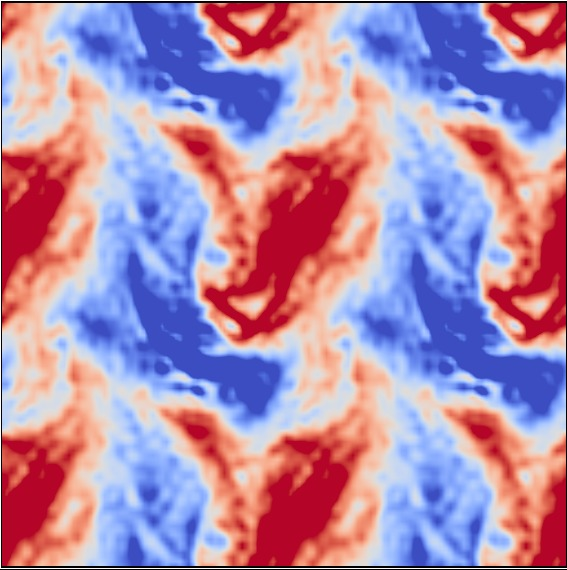
\includegraphics[width=0.2\textwidth]{Figures/ABC/t1z64.jpeg}} & \subfloat[z = 128]{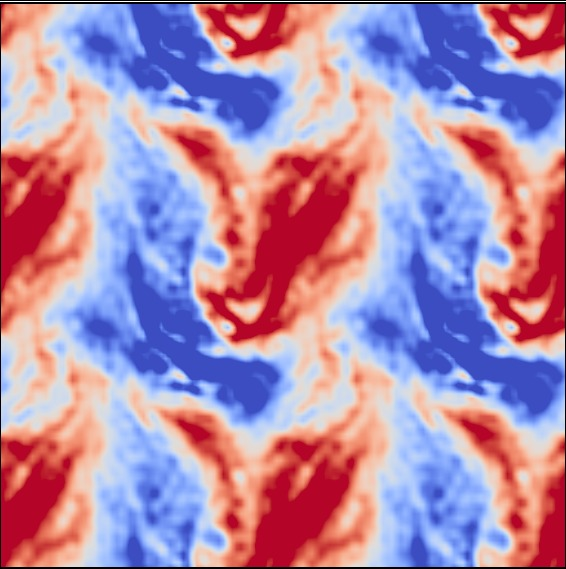
\includegraphics[width=0.2\textwidth]{Figures/ABC/t1z127.jpeg}} \\
\subfloat[z = 1]{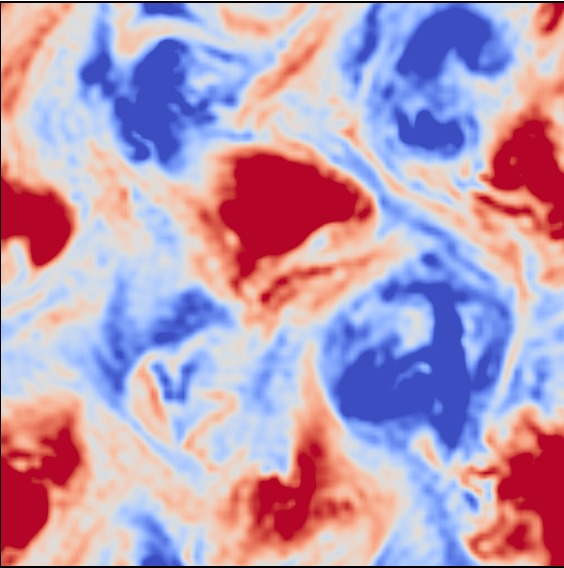
\includegraphics[width=0.2\textwidth]{Figures/ABC/t6z0.jpeg}} & \subfloat[z = 33]{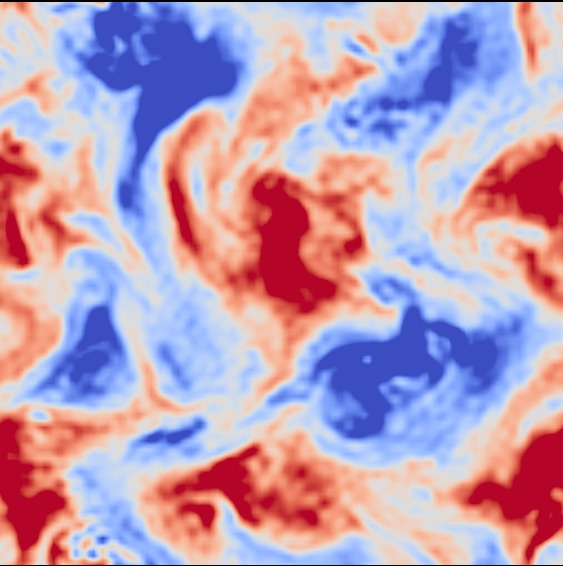
\includegraphics[width=0.2\textwidth]{Figures/ABC/t6z32.jpeg}} & \subfloat[z = 65]{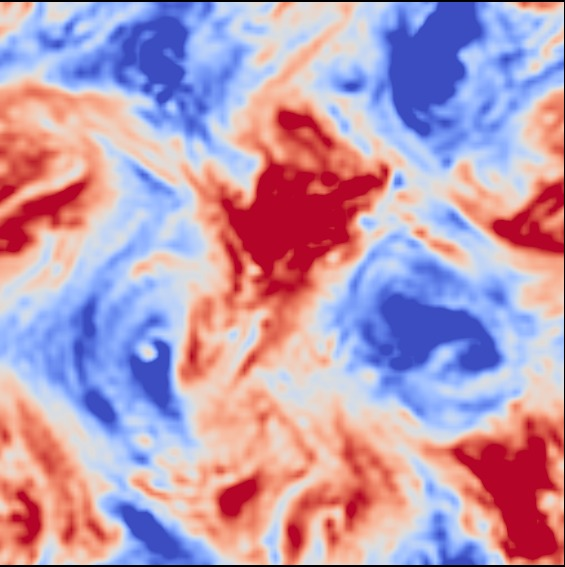
\includegraphics[width=0.2\textwidth]{Figures/ABC/t6z64.jpeg}} & \subfloat[z = 128]{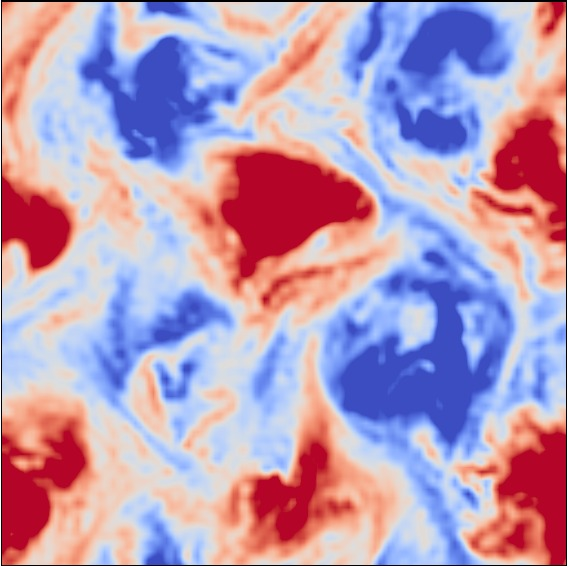
\includegraphics[width=0.2\textwidth]{Figures/ABC/t6z127.jpeg}} \\
\subfloat[z = 1]{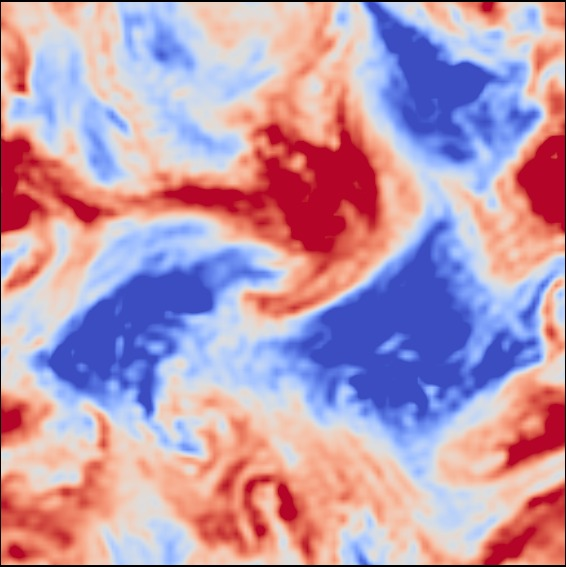
\includegraphics[width=0.2\textwidth]{Figures/ABC/t12z0.jpeg}} & \subfloat[z = 33]{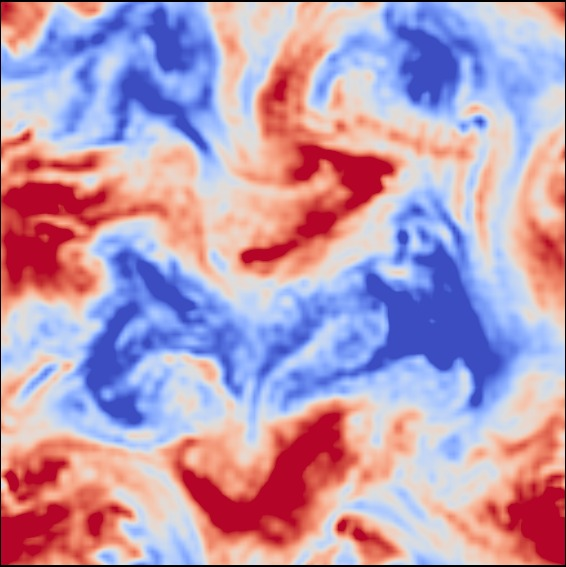
\includegraphics[width=0.2\textwidth]{Figures/ABC/t12z32.jpeg}} & \subfloat[z = 65]{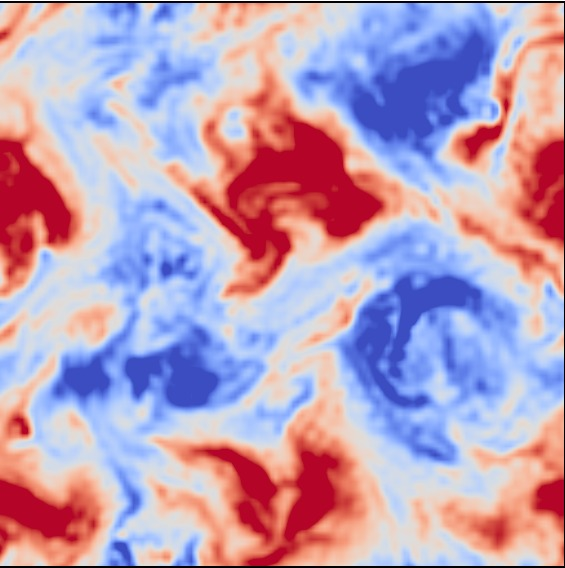
\includegraphics[width=0.2\textwidth]{Figures/ABC/t12z64.jpeg}} & \subfloat[z = 128]{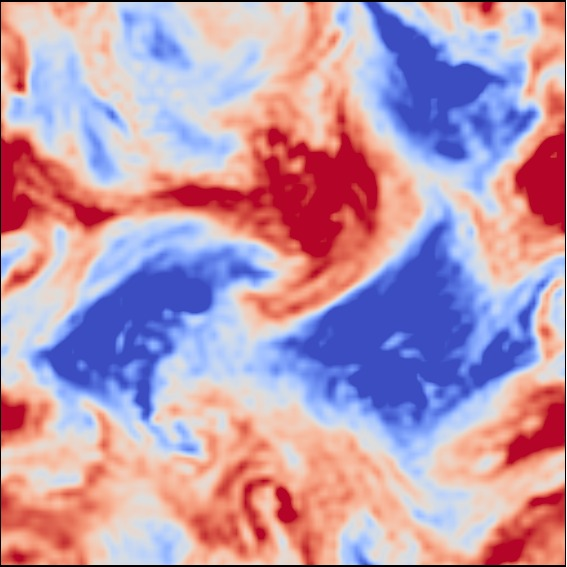
\includegraphics[width=0.2\textwidth]{Figures/ABC/t12z127.jpeg}} \\
\subfloat[z = 1]{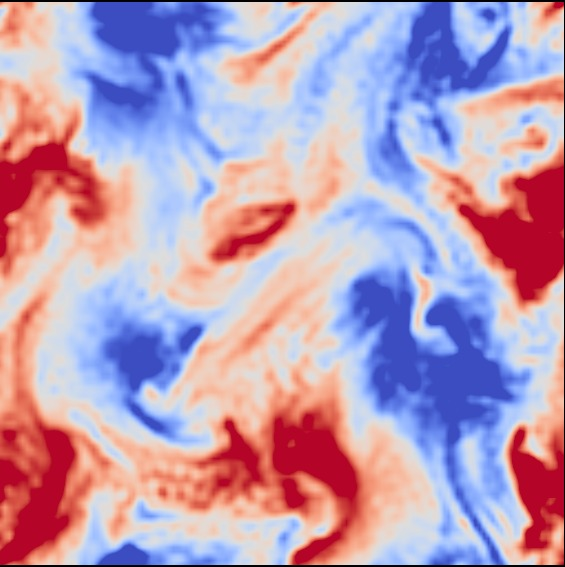
\includegraphics[width=0.2\textwidth]{Figures/ABC/t20z0.jpeg}} & \subfloat[z = 33]{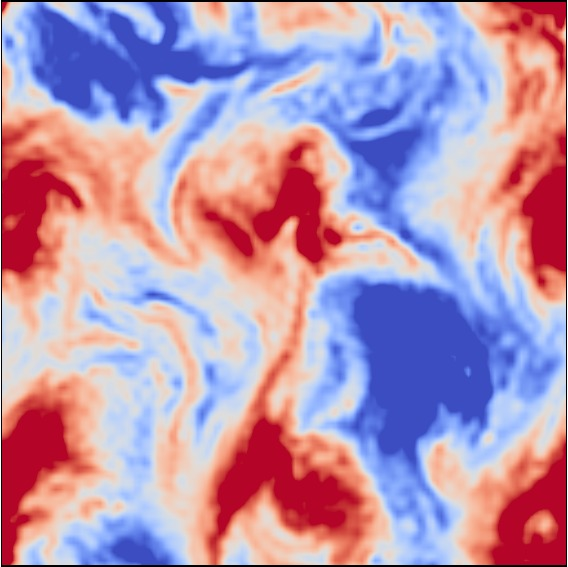
\includegraphics[width=0.2\textwidth]{Figures/ABC/t20z32.jpeg}} & \subfloat[z = 65]{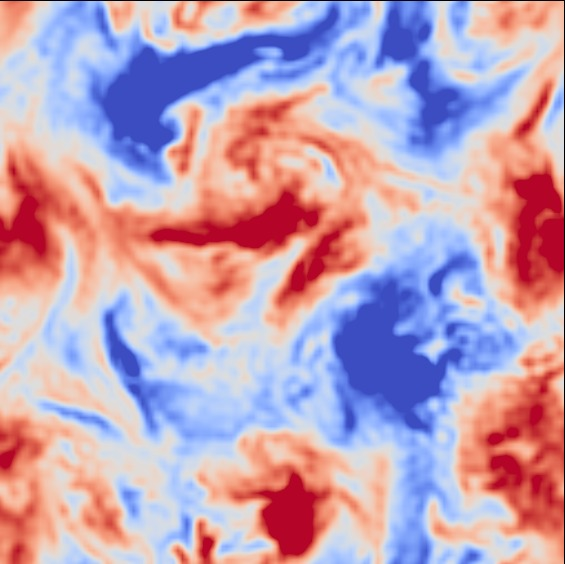
\includegraphics[width=0.2\textwidth]{Figures/ABC/t20z64.jpeg}} & \subfloat[z = 128]{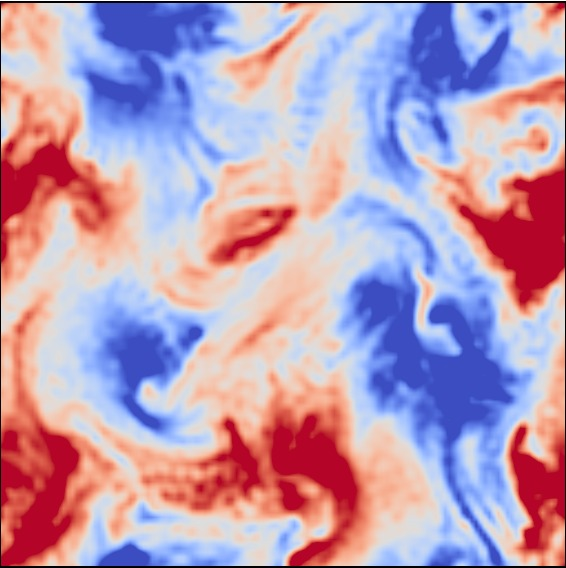
\includegraphics[width=0.2\textwidth]{Figures/ABC/t20z127.jpeg}}

\end{tabular}
\caption{Time Evolution of Velocity field due to ABC forcing. Time increases from top to bottom as $t \in \{15\, s, 90\, s, 180\, s, 300\, s\}$.}
\end{figure}